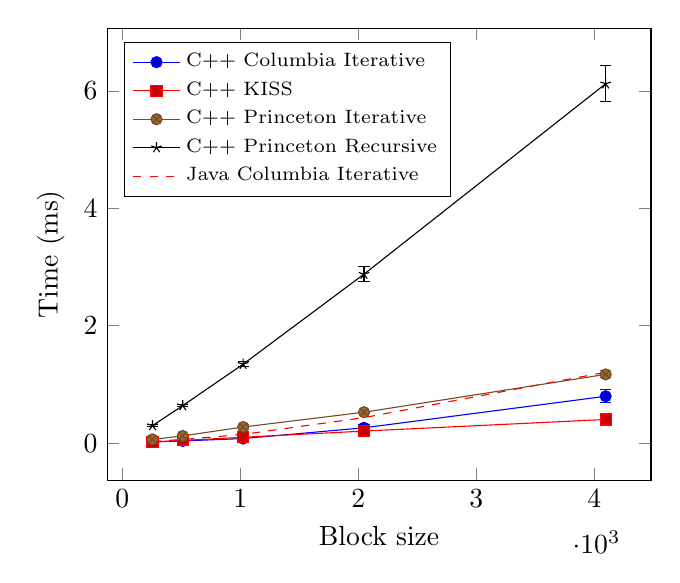
\begin{tikzpicture}
\begin{axis}[xlabel={Block size},ylabel={Time (ms)},width=0.70\linewidth,legend pos=north west,scaled x ticks={base 10:-3},legend cell align=left,legend style={font=\scriptsize}]
\addplot+[error bars/.cd, y dir=both,y explicit] coordinates {
(256, 0.0200) +- (0.0043, 0.0043)
(512, 0.0366) +- (0.0033, 0.0033)
(1024, 0.0773) +- (0.0097, 0.0097)
(2048, 0.2604) +- (0.0634, 0.0634)
(4096, 0.7974) +- (0.1097, 0.1097)
};
\addplot+[error bars/.cd, y dir=both,y explicit] coordinates {
(256, 0.0182) +- (0.0037, 0.0037)
(512, 0.0461) +- (0.0110, 0.0110)
(1024, 0.0992) +- (0.0883, 0.0883)
(2048, 0.2047) +- (0.0765, 0.0765)
(4096, 0.4022) +- (0.0625, 0.0625)
};
\addplot+[error bars/.cd, y dir=both,y explicit] coordinates {
(256, 0.0627) +- (0.0040, 0.0040)
(512, 0.1225) +- (0.0032, 0.0032)
(1024, 0.2744) +- (0.0495, 0.0495)
(2048, 0.5257) +- (0.0185, 0.0185)
(4096, 1.1701) +- (0.0602, 0.0602)
};
\addplot+[error bars/.cd, y dir=both,y explicit] coordinates {
(256, 0.2978) +- (0.0127, 0.0127)
(512, 0.6379) +- (0.0181, 0.0181)
(1024, 1.3437) +- (0.0445, 0.0445)
(2048, 2.8773) +- (0.1288, 0.1288)
(4096, 6.1206) +- (0.3046, 0.3046)
};
\addplot+[style=dashed,color=red,mark=none] coordinates {
(256, 0.0293) +- (0.0042, 0.0042)
(512, 0.0615) +- (0.0047, 0.0047)
(1024, 0.1484) +- (0.0308, 0.0308)
(2048, 0.4338) +- (0.0806, 0.0806)
(4096, 1.2071) +- (0.1807, 0.1807)
};
\legend{C++ Columbia Iterative , C++ KISS , C++ Princeton Iterative , C++ Princeton Recursive, Java Columbia Iterative}
\end{axis}
\end{tikzpicture}
